\documentclass{article}
\usepackage{tikz}
\usetikzlibrary{decorations.pathreplacing}

\begin{document}
	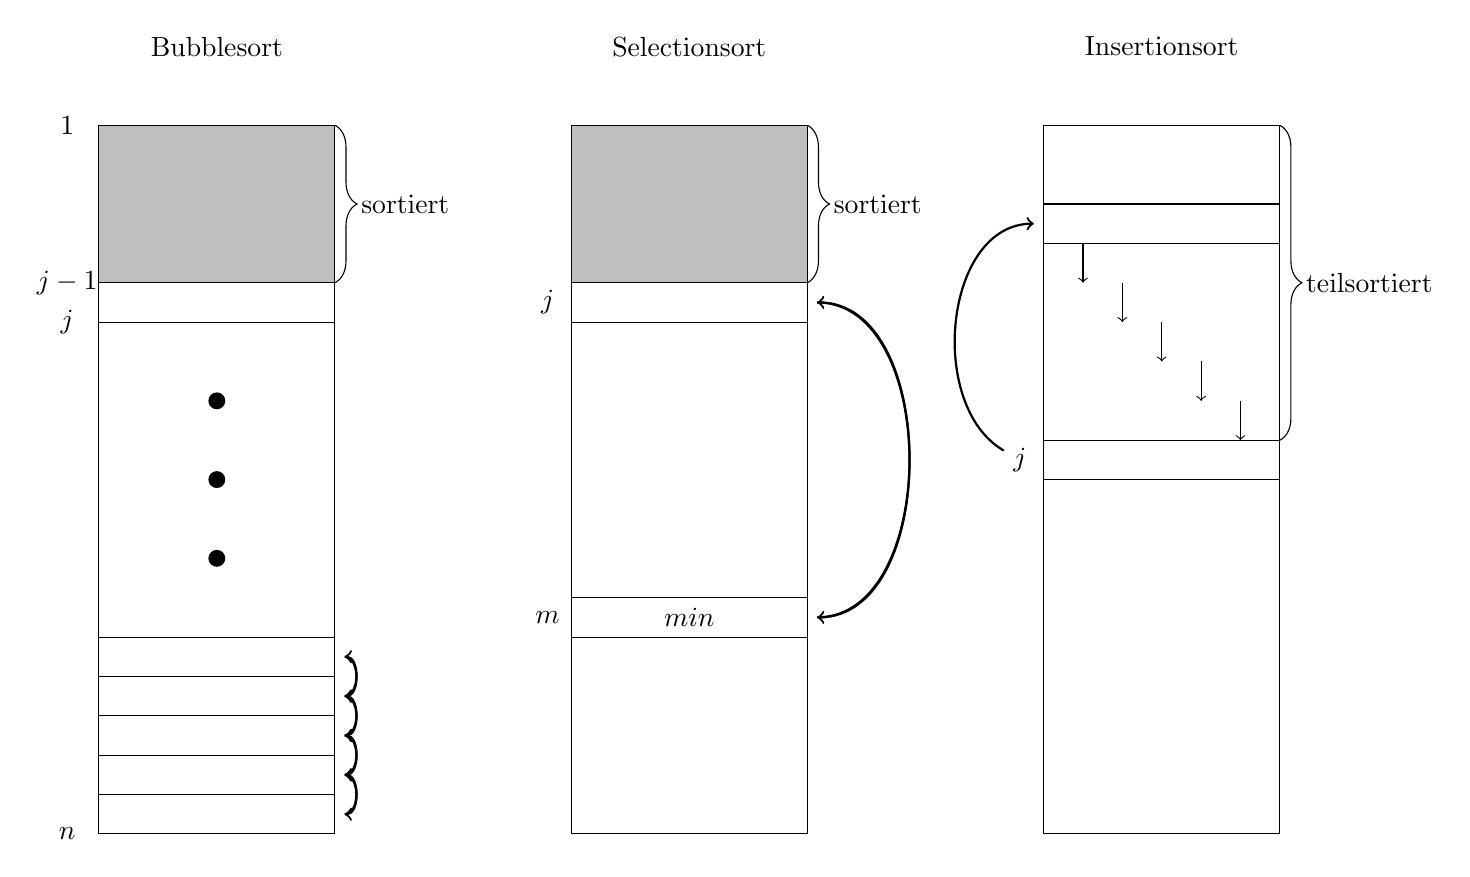
\begin{tikzpicture}
		\node at (1.5,1) (bubble) {Bubblesort};
		\draw (0,0) rectangle (3,-9);
		\draw[fill=lightgray] (0,0) rectangle (3,-2);
		\draw[decorate,decoration={brace,amplitude=8pt}] (3,0) -- (3,-2) node[midway, right, xshift=6pt]{sortiert};
		\draw (0,-2.5) -- (3,-2.5);
		\draw[fill=black] (1.5,-3.5) circle (0.1);
		\draw[fill=black] (1.5,-4.5) circle (0.1);
		\draw[fill=black] (1.5,-5.5) circle (0.1);
		\draw (0,-6.5) -- (3,-6.5);
		\draw (0,-7) -- (3,-7);
		\draw (0,-7.5) -- (3,-7.5);
		\draw (0,-8) -- (3,-8);
		\draw (0,-8.5) -- (3,-8.5);
		
		\node at (-0.4,0) (1) {1};
		\node at (-0.4,-2) (j-1) {$j-1$};
		\node at (-0.4,-2.5) (j) {$j$};
		\node at (-0.4,-9) (n) {$n$};
		
		\node at (3,-6.75) (a) {};
		\node at (3,-7.25) (b) {};
		\node at (3,-7.75) (c) {};
		\node at (3,-8.25) (d) {};
		\node at (3,-8.75) (e) {};
		\draw[->, thick] (a) to [out=0, in=0] (b);
		\draw[->, thick] (b) to [out=0, in=0] (c);
		\draw[->, thick] (c) to [out=0, in=0] (d);
		\draw[->, thick] (d) to [out=0, in=0] (e);
		\draw[->, thick] (e) to [out=0, in=0] (d);
		\draw[->, thick] (d) to [out=0, in=0] (c);
		\draw[->, thick] (c) to [out=0, in=0] (b);
		\draw[->, thick] (b) to [out=0, in=0] (a);
		
		\node at (7.5,1) (selection) {Selectionsort};
		\draw (6,0) rectangle (9,-9);
		\draw[fill=lightgray] (6,0) rectangle (9,-2);
		\draw[decorate,decoration={brace,amplitude=8pt}] (9,0) -- (9,-2) node[midway, right, xshift=6pt]{sortiert};
		\draw (6,-2.5) -- (9,-2.5);
		\node at (5.7,-2.25) (j) {$j$};
		\draw (6,-6.5) -- (9,-6.5);
		\node at (5.7,-6.25) (m) {$m$};
		\draw (6,-6) -- (9,-6);
		\node at (7.5,-6.25) (min) {$min$};
		
		\node at (9,-2.25) (g) {};
		\node at (9,-6.25) (h) {};
		\draw[->,thick] (h) to [out=0, in=0] (g);
		\draw[->,thick] (g) to [out=0, in=0] (h);
		
		\node at (13.5,1) (insert) {Insertionsort};
		\draw (12,0) rectangle (15,-9);
		\draw[decorate,decoration={brace,amplitude=8pt}] (15,0) -- (15,-4) node[midway, right, xshift=6pt]{teilsortiert};
		\draw (12,-4.5) -- (15,-4.5);
		\node at (11.7,-4.25) (j) {$j$};
		\draw (12,-4) -- (15,-4);
		\draw (12,-1) -- (15,-1);
		\draw (12,-1.5) -- (15,-1.5);
		\node at (12,-1.25) (k) {};
		\draw[->,thick] (j) to [out=150, in=180] (k);
		
		\draw[->] (12.5,-1.5) -- (12.5,-2);
		\draw[->] (13,-2) -- (13,-2.5);
		\draw[->] (13.5,-2.5) -- (13.5,-3);
		\draw[->] (14,-3) -- (14,-3.5);
		\draw[->] (14.5,-3.5) -- (14.5,-4);
	\end{tikzpicture}
\end{document}